\section{Motivation}   % Motivation

\begin{frame}
  \frametitle{Theoretical GFLOP/s: GPU vs. CPU}	
  \begin{columns}
  \column{0.9\textwidth}
    \begin{figure}[H]
       \centering
            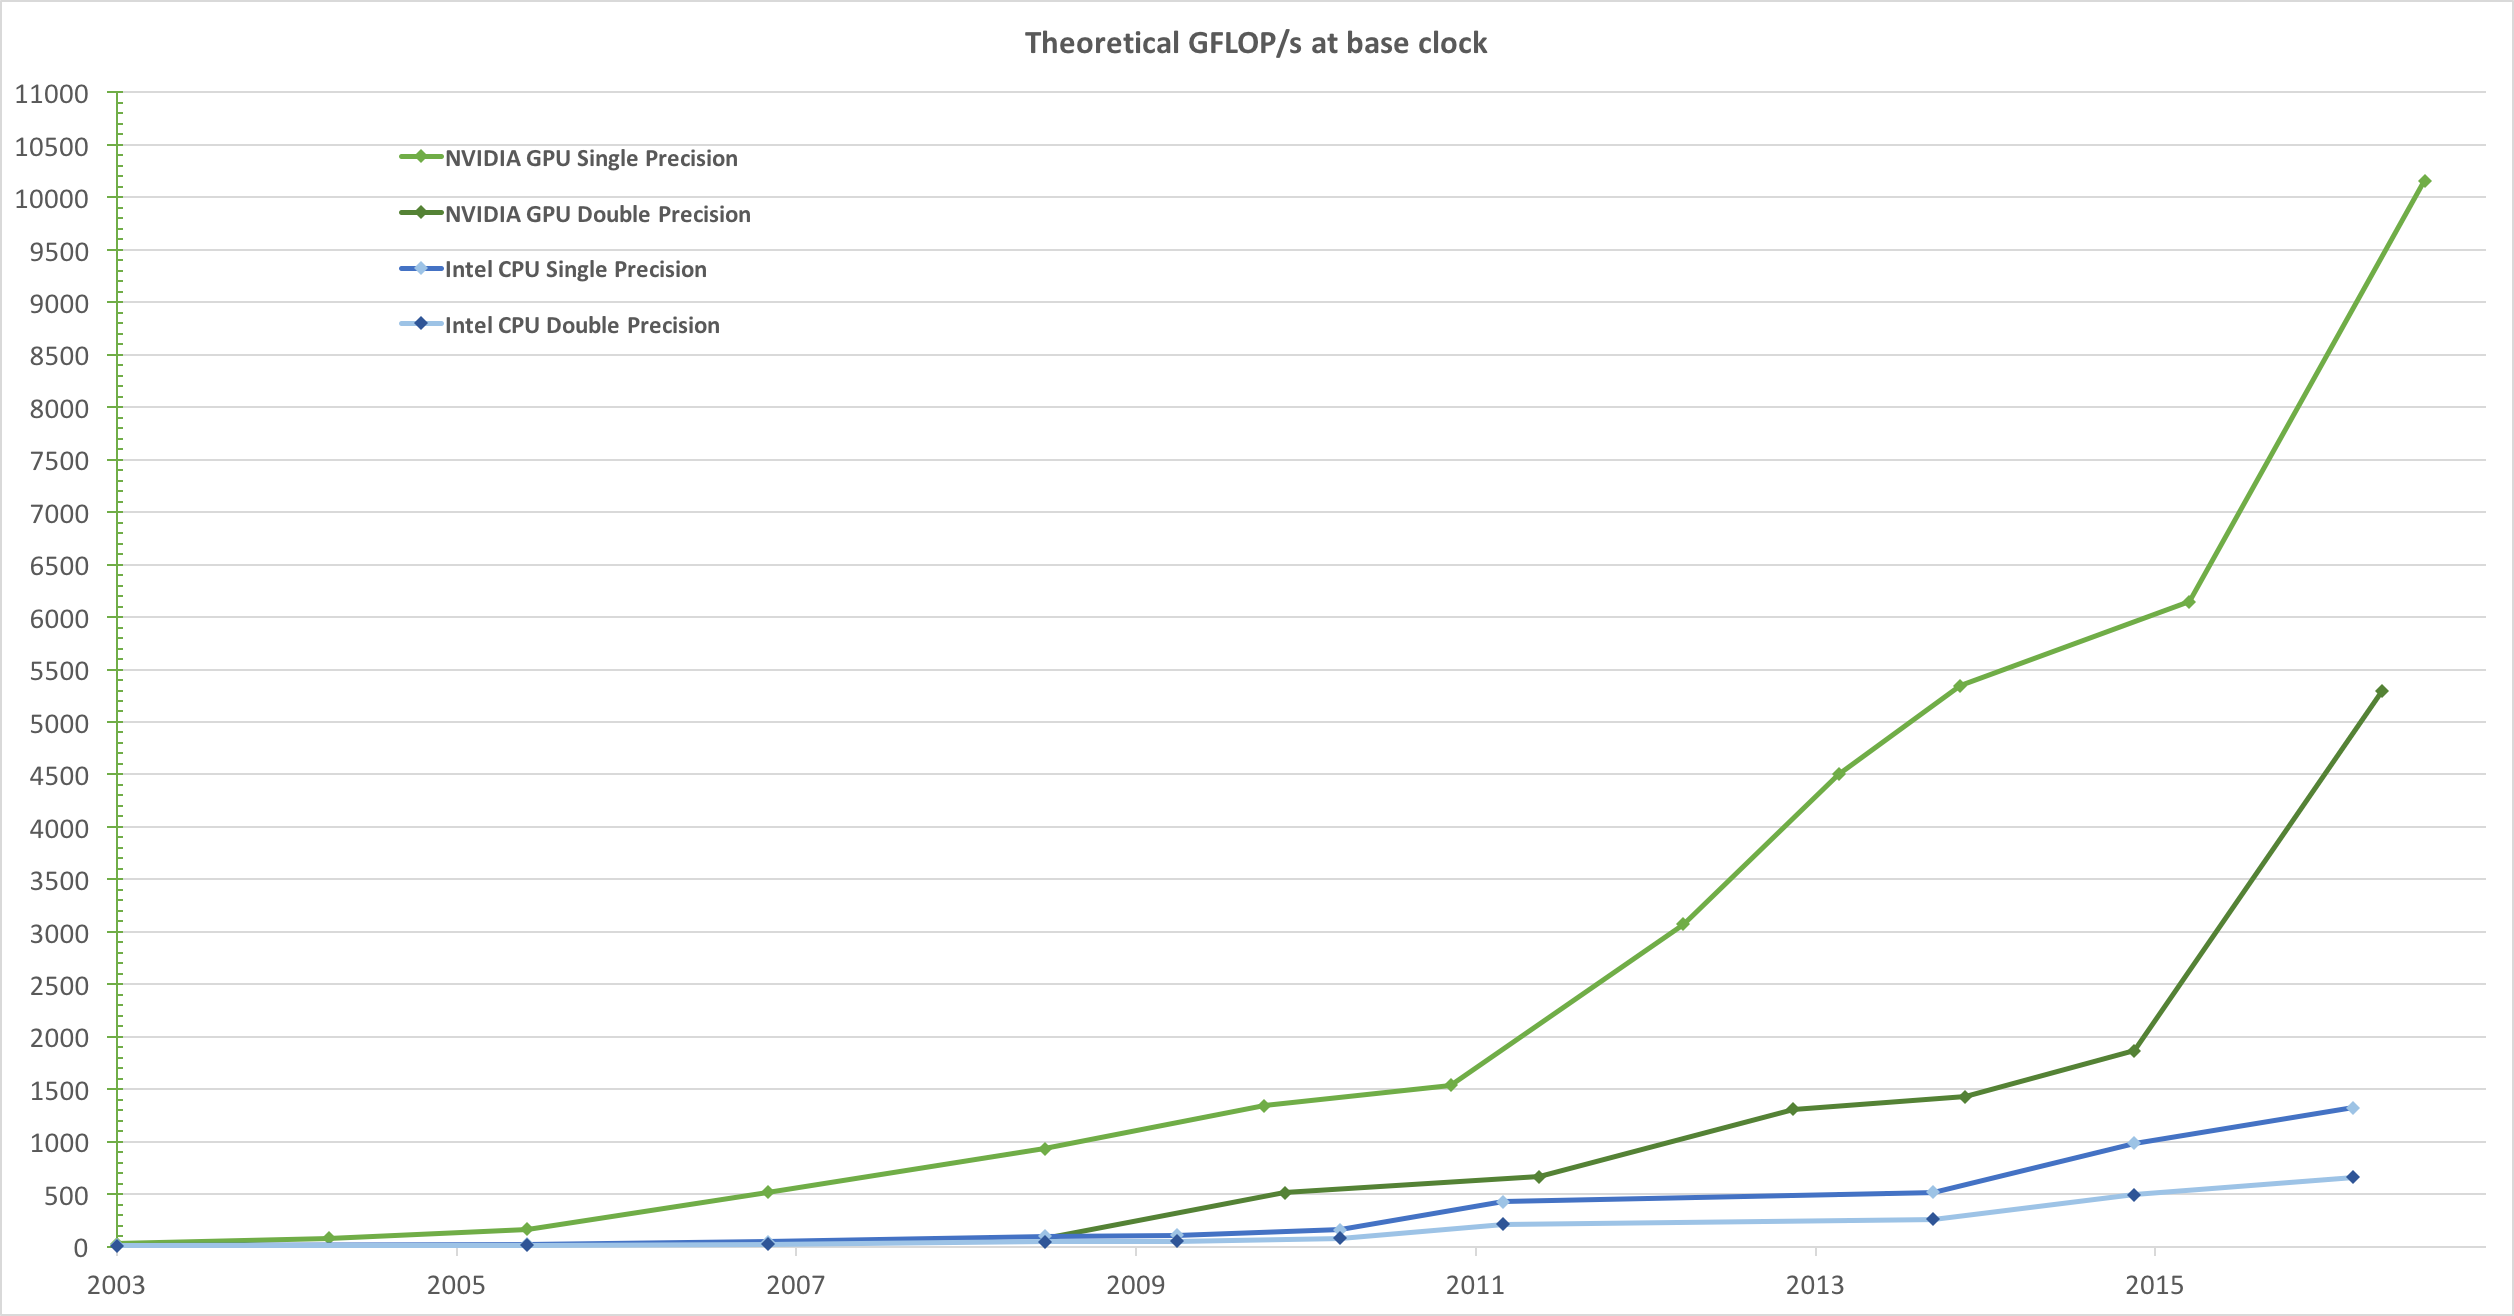
\includegraphics[width=0.90\textwidth]{./img/theoretical-gflops.png}
	    \caption{\small{Theoretical GFLOP/s: GPUs vs. CPUs.\newline\footnote{https://docs.nvidia.com/cuda/archive/9.1/pdf/CUDA\_C\_Programming\_Guide.pdf}}}
     \end{figure}
     \end{columns}

\end{frame}	

\begin{frame}
	\frametitle{CPU processor trend (last 50 years)}
  \begin{columns}
  \column{0.9\textwidth}
    \begin{figure}[H]
       \centering
            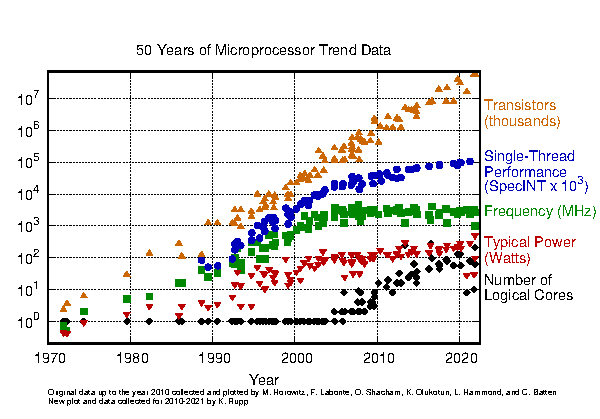
\includegraphics[width=0.80\textwidth]{./img/50-years-processor-trend.pdf}
     \end{figure}
     \end{columns} 
      \begin{itemize} 
         \item After the year $2000$, \texttt{freq.}/\texttt{power} 
		 for a single CPU core reaches a max. (\textcolor{red}{\textbf{Heat dissipation!}}).
      \end{itemize}
\end{frame} 

\begin{frame}
	\frametitle{Energy efficiency per job: GPU vs. CPU}
  \begin{columns}
  \column{0.9\textwidth}
    \begin{figure}[H]
       \centering
            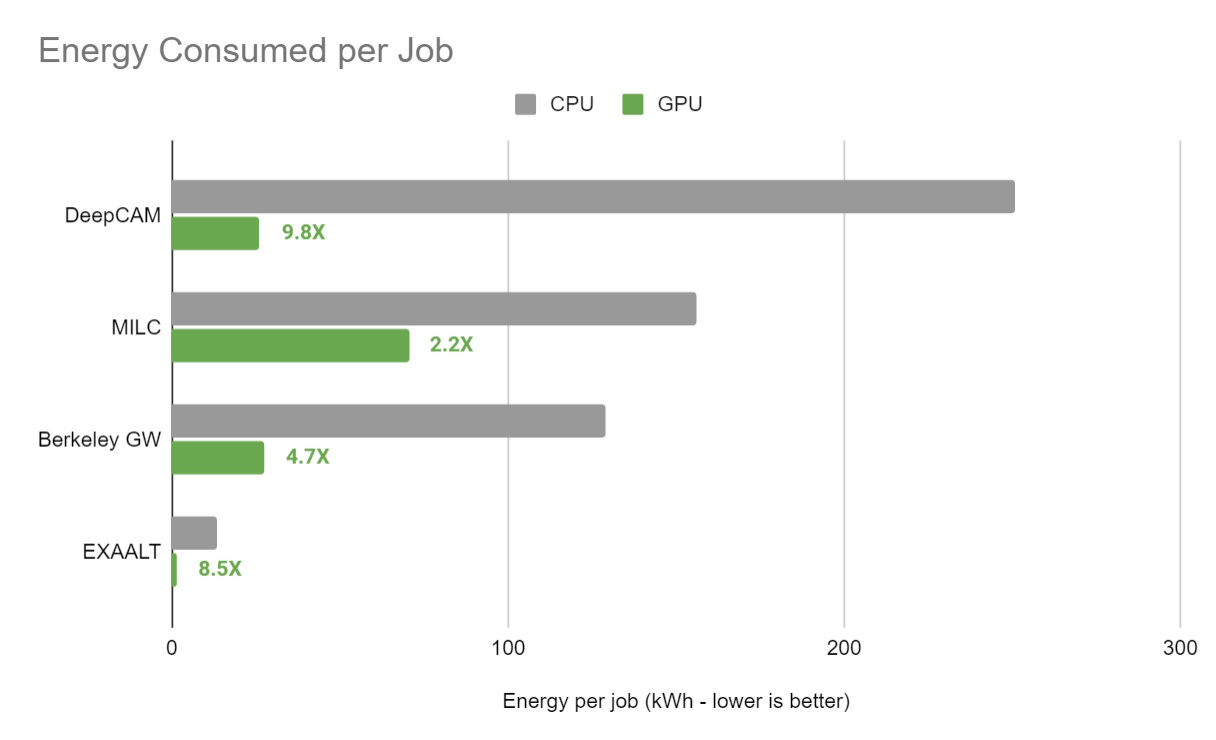
\includegraphics[width=0.80\textwidth]{./img/NERSC-energy-efficiency-findings.jpg} 
	    \caption{\small{Energy efficiency per job (NERSC).\newline\footnote{https://blogs.nvidia.com/blog/gpu-energy-efficiency-nersc/ (05/21/2023)}}}
     \end{figure}
     \end{columns}
\end{frame}
